% Aufgabe: Messaufgaben auflisten
% Vorbereitung: Vorbereitungsaufgaben bearbeiten
% Versuchsaufbau: Verwendete Apparatur, Beschreibung Funktionsweise/Nutzen mit Skizze/Foto

\vfill

\section{Aufgabe}
Zielsetzung dieser Versuchsreihe ist die Untersuchung des Verhaltens eines RC\hspace{0.15ex}-Kreises
in Abhängigkeit von Zeit, Frequenz und Phase. Speziell soll anhand der beobachteten Beziehungen
die Zeitkonstante $\tau$ bestimmt werden. Dazu werden entsprechende Messungen durchgeführt und
aufbauend auf den theoretischen Grundlagen ausgewertet.

\newpage

\section{Durchführung}
\label{sec:durchführung}

\begin{figure}
	\centering
	\vspace{1.23ex}
	\resizebox{0.93\width}{!}{\begin{tikzpicture}\tikzstyle{every node} = [font = \small]

\ctikzset{bipoles/thickness = 1}
\ctikzset{bipoles/length = 1cm}

\begin{scope}[line width = 1pt]
	% Frequenzmesser
	\draw
		(0,-1) to[short]
		++(-3,0) to[rmeter, t=\raisebox{-0.6ex}{$\hspace{-0.1ex}\small\nu$}]
		++(0,4) to[short]
		++(3,0);

	% Funktionsgenerator
	\draw
		(0,-1) to[short, *-o] ++(0,0.55);
	\draw
		(-0.2,-0.25) to[short, o-]
		++(0,0.2) to[short]
		++(-0.55,0) to[sV]
		++(0,1) to[short]
		++(0.55,0) to[short, -o]
		++(0,0.2);
	\draw
		(0,-0.25) to[tV, o-o] ++(0,1.4);
	\draw
		(0.2,-0.25) to[short, o-]
		++(0,0.2) to[short]
		++(0.55,0) to[sqV]
		++(0,1) to[short]
		++(-0.55,0) to[short, -o]
		++(0,0.2);
	\draw
		(0,1.35) to[R, o-, l=$R_0$]
		++(0,1.4) to[short, -*]
		++(0,0.25);
	
	% RC-Glied
	\draw
		(0,3) to[R, -*, l_=$R$]
		++(3,0) to[C, -*, l_=\raisebox{-0.2ex}{$C$}]
		++(0,-4) to[short]
		++(-3,0);

	% Oszillograph
	\draw
		(3,3) to[short]
		++(3,0) to[short]
		++(0,-1.7);
	\draw
		(5.85,1.3) -- ++(0.3,0);
	\draw
		(5.85,0.7) -- ++(0.3,0);
	\draw
		(6,0.7) to[short, -*]
		++(0,-1.7) -- ++(0,-0.3);
	\draw
		(5.8,-1.3) -- ++(0.4,0);
	\draw
		(5.865,-1.375) -- ++(0.27,0);
	\draw
		(5.925,-1.45) -- ++(0.15,0);
	\draw
		(0,3) to[short]
		++(0,0.75) to[short]
		++(6.75,0) to[short]
		++(0,-2.45);
	\draw
		(6.6,1.3) -- ++(0.3,0);
	\draw
		(6.6,0.7) -- ++(0.3,0);
	\draw
		(6.75,0.7) to[short]
		++(0,-1.7) to[short]
		++(-3.75,0);
	\draw
		(5.125,-1) to[short, *-]
		++(0,2) to[short]
		++(0.5,0);
	\draw
		(5.625,0.85) -- ++(0,0.3);
	\draw
		(7.125,0.85) -- ++(0,0.3);
	\draw
		(7.125,1) to[short, -*]
		++(0.5,0);
	\draw[rounded corners=3mm]
		(5.525,1.4) -- ++(1.7,0) -- ++(0,-0.8) -- ++(-1.7,0) -- cycle;

	\node at (5.5,1.7) {CH\hspace{0.3ex}1};
	\node at (7.25,1.7) {CH\hspace{0.3ex}2};

	\node[rotate=270] at (8,1) {Oszillograph};
	\node[rotate=90] at (-3.6,1) {Frequenzmesser};
	\node at (0,-1.325) {Funktionsgenerator};
\end{scope}
\end{tikzpicture}}
	\vspace{1.23ex}
	\caption{Veranschaulichendes Schaltbild des Messaufbaus.}
	\label{fig:circuit}
\end{figure}

Zunächst soll der Entladungsvorgang des Kondensators nach \eqref{eqn:entladung_spannung} betrachtet werden.
Am Funktionsgenerator in Abbildung \ref{fig:circuit} wird dazu ein Rechtecksignal eingestellt. Durch Wahl
einer ausreichend großen Periode $T \gg \tau$ fällt die Kondensatorspannung am Eingang \mbox{CH\hspace{0.3ex}1}
gegen Null ab. Auf diesem Weg lässt sich die Messskala kalibrieren. Anschließend wird unter erhöhter Frequenz
ein Druck des Oszilloskopschirms angefertigt, um aus den vom Verlauf abzulesenden Daten die Zeitkonstante
$\tau$ zu bestimmen. Im Weiteren erlaubt das Abgreifen einer veränderlichen Sinusspannung, über das
\mbox{Transmissionsverhalten~\eqref{eqn:transmission} auf} $\tau = RC$ zu schließen. Die Amplitude der
Kondensatorspannung wird hierbei mit den entsprechenden Frequenzen nachgehalten. Darauf folgend ist die
Phasenabhängigkeit~\eqref{eqn:phase} zu untersuchen. Es werden Verlauf von Eingangsspannung
an CH\hspace{0.3ex}2 und Ausgangsspannung an CH\hspace{0.3ex}1 gemeinsam betrachtet, um daraus die
Verschiebung
\begin{equation}
	\varphi = \pfrac{a}{b} \, \qty{360}{\degree}
\end{equation}
mit den Größen $a$ und $b$ nach Abbildung \ref{fig:ab} zu erhalten. 

\begin{figure}
	\centering
	\vspace{0.615ex}
	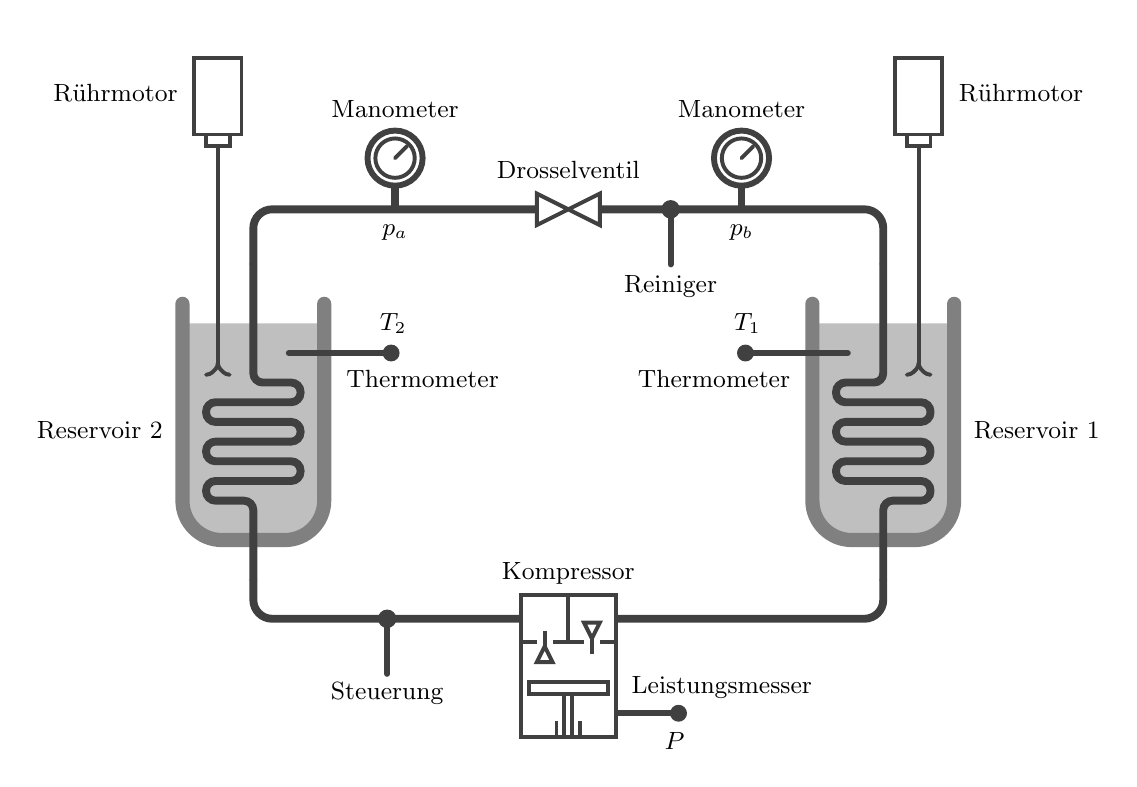
\begin{tikzpicture}
		\tikzstyle{every node} = [font = \small]

% frame
\draw[draw=white] 
	(0,0) -- ++(0,9) -- ++(8,0) -- ++(0,-9) -- cycle;

% valve
\draw[draw=darkgray, line width=0.5mm] 
	(3.6,6.7) -- ++(0,-0.2) -- ++(0.8,0.4) -- ++(0,-0.4) -- ++(-0.8,0.4) -- cycle;

% compresser
\draw[draw=darkgray, line width=0.5mm] 
	(3.4,0) -- ++(0,1.8) -- ++(1.2,0) -- ++(0,-1.8) -- cycle;
\draw[draw=darkgray, line width=0.5mm] 
	(4,1.8) -- ++(0,-0.6);
\draw[draw=darkgray, line width=0.5mm] 
	(3.8,1.2) -- ++(0.4,0);
\draw[draw=darkgray, line width=0.5mm] 
	(3.4,1.2) -- ++(0.2,0);
\draw[draw=darkgray, line width=0.5mm] 
	(4.6,1.2) -- ++(-0.2,0);
\draw[draw=darkgray, line width=0.5mm] 
	(3.7,1.35) -- ++(0,-0.2);
\draw[draw=darkgray, line width=0.5mm] 
	(3.7,1.15) -- ++(-0.1,-0.2) -- ++(0.2,0) -- cycle;
\draw[draw=darkgray, line width=0.5mm] 
	(4.3,1.25) -- ++(0,-0.2);
\draw[draw=darkgray, line width=0.5mm] 
	(4.3,1.25) -- ++(-0.1,0.2) -- ++(0.2,0) -- cycle;
\draw[draw=darkgray, line width=0.5mm] 
	(3.5,0.7) -- ++(1,0) -- ++(0,-0.15) -- ++(-1,0) -- cycle;
\draw[draw=darkgray, line width=0.5mm] 
	(3.95,0.55) -- ++(0,-0.55);
\draw[draw=darkgray, line width=0.5mm] 
	(4.05,0.55) -- ++(0,-0.55);
\draw[draw=darkgray, line width=0.5mm] 
	(3.85,0.2) -- ++(0,-0.2);
\draw[draw=darkgray, line width=0.5mm] 
	(4.15,0.2) -- ++(0,-0.2);

% wattmeter
\draw[draw=darkgray, line width=0.75mm] 
	(4.6,0.3) -- (5.4,0.3);
\draw[draw=darkgray, fill=darkgray] 
	(5.4,0.3) circle (1mm);

% control
\draw[draw=darkgray, line width=0.75mm, line cap=round] 
	(1.7,1.5) -- (1.7,0.8);
\draw[draw=darkgray, fill=darkgray] 
	(1.7,1.5) circle (1.1mm);

% diffuser
\draw[draw=darkgray, line width=0.75mm, line cap=round] 
	(5.3,6.7) -- (5.3,6);
\draw[draw=darkgray, fill=darkgray] 
	(5.3,6.7) circle (1.1mm);

% left

% bucket
\draw[draw=lightgray, fill=lightgray, line width=0mm, line cap=round, rounded corners=5mm] 
	(-0.9,5.25) -- ++(0,-2.75) -- ++(1.8,0) -- ++(0,2.75);
\draw[draw=gray, line width=1.8mm, line cap=round, rounded corners=5mm] 
	(-0.9,5.5) -- ++(0,-3) -- ++(1.8,0) -- ++(0,3);
% mixer
\draw[draw=darkgray, line width=0.5mm] 
	(-0.45,7.5) -- ++(0,-2.75);
\draw[draw=darkgray, line width=0.5mm, line cap=round, rounded corners=0.45mm] 
	(-0.45,4.75) -- ++(0,-0.05) -- ++(-0.1,-0.1) -- ++(-0.05,0);
\draw[draw=darkgray, line width=0.5mm, line cap=round, rounded corners=0.45mm] 
	(-0.45,4.75) -- ++(0,-0.05) -- ++(0.1,-0.1) -- ++(0.05,0);
\draw[draw=darkgray, line width=0.5mm] 
	(-0.6,7.65) -- ++(0,-0.15) -- ++(0.3,0) -- ++(0,0.15);
\draw[draw=darkgray, line width=0.5mm] 
	(-0.75,7.65) -- ++(0.6,0) -- ++(0,0.975) -- ++(-0.6,0) -- cycle;
% thermometer
\draw[draw=darkgray, line width=0.75mm, line cap=round] 
	(0.45,4.875) -- (1.75,4.875);
\draw[draw=darkgray, fill=darkgray] 
	(1.75,4.875) circle (1mm);
% manometer
\draw[draw=darkgray, line width=1mm] 
	(1.8,6.7) -- (1.8,7);
\draw[draw=darkgray, line width=0.75mm] 
	(1.8,7.35) circle (3.5mm);
\draw[draw=darkgray, line width=0.5mm] 
	(1.8,7.35) circle (2.5mm);
\draw[draw=darkgray, line width=0.5mm, line cap=round] 
	(1.8,7.35) -- ++(0.15,0.15);
% snake
\draw[draw=darkgray, line width=1mm, line cap=round, rounded corners=1.2mm] 
	(0,6) -- ++(0,-1.5) -- ++(0.6,0) -- ++(0,-0.25) -- ++(-1.2,0) -- ++(0,-0.25)
	-- ++(1.2,0) -- ++(0,-0.25) -- ++(-1.2,0) -- ++(0,-0.25)
	-- ++(1.2,0) -- ++(0,-0.25) -- ++(-1.2,0) -- ++(0,-0.25)
	-- ++(0.6,0) -- (0,2);
\draw[draw=darkgray, line width=1mm, rounded corners=2.4mm] 
	(0,2) -- (0,1.5) -- (3.4,1.5);
\draw[draw=darkgray, line width=1mm, rounded corners=2.4mm] 
	(0,6) -- (0,6.7) -- (3.6,6.7);

% right

% bucket
\draw[draw=lightgray, fill=lightgray, line width=0mm, line cap=round, rounded corners=5mm] 
	(7.1,5.25) -- ++(0,-2.75) -- ++(1.8,0) -- ++(0,2.75);
\draw[draw=gray, line width=1.8mm, line cap=round, rounded corners=5mm] 
	(7.1,5.5) -- ++(0,-3) -- ++(1.8,0) -- ++(0,3);
% mixer
\draw[draw=darkgray, line width=0.5mm] 
	(8.45,7.5) -- ++(0,-2.75);
\draw[draw=darkgray, line width=0.5mm, line cap=round, rounded corners=0.45mm] 
	(8.45,4.75) -- ++(0,-0.05) -- ++(-0.1,-0.1) -- ++(-0.05,0);
\draw[draw=darkgray, line width=0.5mm, line cap=round, rounded corners=0.45mm] 
	(8.45,4.75) -- ++(0,-0.05) -- ++(0.1,-0.1) -- ++(0.05,0);
\draw[draw=darkgray, line width=0.5mm] 
	(8.3,7.65) -- ++(0,-0.15) -- ++(0.3,0) -- ++(0,0.15);
\draw[draw=darkgray, line width=0.5mm] 
	(8.15,7.65) -- ++(0.6,0) -- ++(0,0.975) -- ++(-0.6,0) -- cycle;
% thermometer
\draw[draw=darkgray, line width=0.75mm, line cap=round] 
	(7.55,4.875) -- (6.25,4.875);
\draw[draw=darkgray, fill=darkgray] 
	(6.25,4.875) circle (1mm);
% manometer
\draw[draw=darkgray, line width=1mm] 
	(6.2,6.7) -- (6.2,7);
\draw[draw=darkgray, line width=0.75mm] 
	(6.2,7.35) circle (3.5mm);
\draw[draw=darkgray, line width=0.5mm] 
	(6.2,7.35) circle (2.5mm);
\draw[draw=darkgray, line width=0.5mm, line cap=round] 
	(6.2,7.35) -- ++(0.15,0.15);
% snake
\draw[draw=darkgray, line width=1mm, line cap=round, rounded corners=1.2mm] 
	(8,6) -- ++(0,-1.5) -- ++(-0.6,0) -- ++(0,-0.25) -- ++(1.2,0) -- ++(0,-0.25)
	-- ++(-1.2,0) -- ++(0,-0.25) -- ++(1.2,0) -- ++(0,-0.25)
	-- ++(-1.2,0) -- ++(0,-0.25) -- ++(1.2,0) -- ++(0,-0.25)
	-- ++(-0.6,0) -- (8,2);
\draw[draw=darkgray, line width=1mm, rounded corners=2.4mm] 
	(8,2) -- (8,1.5) -- (4.6,1.5);
\draw[draw=darkgray, line width=1mm, rounded corners=2.4mm] 
	(8,6) -- (8,6.7) -- (4.4,6.7);

% labels
\node at (-1.75,8.175) {Rührmotor};
\node at (9.75,8.175) {Rührmotor};
\node at (1.8,7.975) {Manometer};
\node at (6.2,7.975) {Manometer};
\node at (4,7.2) {Drosselventil};
\node at (1.8,6.4) {$p_a$};
\node at (6.2,6.4) {$p_b$};
\node at (5.3,5.725) {Reiniger};
\node at (1.775,5.25) {$T_2$};
\node at (6.275,5.25) {$T_1$};
\node at (2.15,4.55) {Thermometer};
\node at (5.85,4.55) {Thermometer};
\node at (-1.95,3.9) {Reservoir $2$};
\node at (9.95,3.9) {Reservoir $1$};
\node at (4,2.075) {Kompressor};
\node at (1.7,0.55) {Steuerung};
\node at (5.95,0.625) {Leistungsmesser};
\node at (5.35,-0.05) {$P$};

	\end{tikzpicture}
	\vspace{1.23ex}
	\caption{Schematische Darstellung des Oszillographenschirms.}
	\label{fig:ab}
\end{figure}

Anhand der so gewonnenen Messwerte wird zur Phase auch eine Polarprojektion des Zusammenhangs
\eqref{eqn:amplitude_phase} vorgenommen. Zuletzt ist noch die Integralfunktion des
RC\hspace{0.15ex}-Gliedes qualitativ anhand verschiedener Signaltypen abgebildet.
